\documentclass{cours}
\usepackage{pgfplots}
\usepackage{multicol}
\usepackage{amssymb}
\usepackage{xr}
\usepackage{fontawesome}
\usetikzlibrary {decorations.text, backgrounds, intersections}
\usepackage{mhchem}

\begin{document}

\tikzset{directed/.style={
  postaction={decorate,
              decoration={markings, % arrows on the field lines
                          mark=at position 0.1 with {\draw[-stealth](-1pt,0) -- (1pt,0);}
                         }
             }
   }
   }

\setcounter{chapter}{22}
\chapter{Le champ magnétique}

\section{Définition}%
\label{sec:definition}

Le champ magnétique est une grandeur vectorielle qui permet de caractériser les effets magnétiques (courants, aimants permanents). Le champ magnétique est généralement noté $\vv{B}$ et s'exprime en tesla (T) (d'après Nikola Tesla 1856--1943). 

Le champ magnétique $\vv{B}(\vv{r})$ est défini en tout point de l'espace, c'est un \emph{champ vectoriel}. 

\section{Représentation}%
\label{sec:representation}

On représente le champ magnétique dans l'espace par des \emph{lignes de champ} qui sont en tout point tangentes au vecteur champ magnétique.

\begin{center}
  \includegraphics[width=8cm]{images/carte_champ_b.pdf}
  \captionof{figure}{Carte de champ magnétique d'un aimant doit ou d'une bobine longue. Le champ est le plus intense au centre de la figure car les lignes de champ y sont très resserrées et il y est aussi homogène car les lignes de champ sont parallèles.}
\end{center}
D'une carte de champ magnétique, on peut déduire des informations sur le vecteur champ magnétique :
\begin{itemize}
  \item Le champ magnétique est uniforme lorsque des lignes de champ sont parallèles ; 
  \item lorsque les lignes de champ se resserrent, le champ magnétique augmente ;
  \item les lignes de champ magnétique sont des courbes fermées qui ne peuvent pas se croiser. Les boucles formées par les lignes de champ entourent les sources du champ magnétique.
\end{itemize}

\section{Sources de champ magnétique}%
\label{sec:sources_de_champ_magnetique}
\subsection{Les aimants permanents}%
\label{sub:les_aimants_permanents}

Un aimant permanent est un matériau qui produit spontanément un champ magnétique. Il possède un pôle nord et un pôle sud, les lignes de champ à l'extérieur de l'aimant vont du pôle nord vers le pôle sud. Le champ magnétique à proximité d'un aimant permanent peut aller jusqu'à environ \SI{1}{\tesla}. Le champ magnétique est créé par les moments magnétiques atomiques des atomes qui composent le matériau de l'aimant.

\begin{center}
  \begin{tikzpicture}
  %tikz  magnetisme
\tikzstyle directed=[postaction={decorate,decoration={markings, % arrows on the field lines
  mark=at position .1 with {\arrowreversed[scale=1.5]{stealth}},
  mark=at position .9 with {\arrowreversed[scale=1.5]{stealth}}}}]
\tikzstyle fLines=[directed]

\def\lmag{1.8}  % length of magnet
\def\wmag{0.4}  % thickness of magnet
\def\nc{5}      % no. of lines = 2*\nc+1

\begin{scope}
\coordinate (A) at (-\lmag/2,\wmag/2);
\coordinate (B) at (-\lmag/2,-\wmag/2);
\draw[fill, color=gray](A) rectangle ++(\lmag/2,-\wmag)node[white,midway]{S};
\draw[fill, color=black](0,-\wmag/2) rectangle ++(\lmag/2,\wmag)node[white,midway]{N};

\clip (-5,-3) rectangle (5,3);
\foreach \r in {1,...,\nc}{
\draw[fLines]($(A)-(0,0.5*\r*\wmag/\nc)$) arc(({270-asin(\lmag/(2*\r))}):({-90+asin(\lmag/(2*\r))}):\r);
\draw[fLines]($(B)+(0,0.5*\r*\wmag/\nc)$) arc(({-270+asin(\lmag/(2*\r))}):({90-asin(\lmag/(2*\r))}):\r); }
\draw[fLines] (-\lmag/2,0) -- ++(-6,0);
\draw[fLines] (\lmag/2,0) ++(6,0)--(\lmag/2,0);
\end{scope}
  \end{tikzpicture}
\end{center}

\subsection{Les courants électriques}%
\label{sub:les_courants_electriques}

Une particule chargée en mouvement crée un champ magnétique, donc un courant électrique aussi. Par exemple un fil rectiligne parcouru par une intensité $I$ produit un champ magnétique (hors programme) :
\begin{equation}
  \vv{B}(r) = \frac{\mu_0I}{2\pi r}\vet
\end{equation}
$\mu_0 = \SI[input-symbols=\pi]{4\pi e-7}{\tesla\meter\per\ampere}$ est la perméabilité magnétique du vide (ou constante magnétique). 
\begin{center}
  \begin{tikzpicture} [scale=1.3]
  %tikz  magnetisme
\tikzstyle directed=[postaction={decorate,decoration={markings, % arrows on the field lines
  mark=at position -0.08 with {\arrow[scale=1.5]{stealth}},
  }}]
\tikzstyle fLines=[directed]
    \draw[thick] (0, -1)  -- (0, 0);
    \draw[thick,-Stealth] (0, -0.8) -- ++(0,1pt) node [right]{$I$ };
    \foreach \r in {0.2,0.4,...,1}{
      \draw[directed, gray] (0,0) ellipse[x radius=\r, y radius={0.5*\r}];
    }
    \draw[thick, preaction={draw, line width=3pt, white}] (0,0) -- (0,1);
  \end{tikzpicture}
  \captionof{figure}{Champ magnétique créé par un fil rectiligne.}
\end{center}
Plus l'intensité du courant est élevée, plus le champ magnétique est intense. 

Pour créer un champ magnétique dans une direction donnée, on peut former une \emph{spire de courant}. Il s'agit d'un fil parcouru par un courant $I$ qui forme une boucle. Dans ce cas, sur l'axe de la spire, le champ magnétique créé est orienté suivant l'axe de la spire.

\begin{center}
  \begin{tikzpicture}[scale=0.7]
  %tikz  magnetisme
\tikzstyle directed=[postaction={decorate,decoration={markings, % arrows on the field lines
  mark=at position .1 with {\arrowreversed[scale=1.5]{stealth}},
  }}]
\tikzstyle fLines=[directed]
    \path[clip] (-4,-2.7) rectangle (4,2.7);
    \draw[thick](0,2) arc(90:-90:1 and 2);
    \foreach \y in {0.2,0.4,...,1.8} {
        \draw[gray, preaction={draw, white, line width=2pt}] (0,\y) arc(-90:90:{4*(2-\y)/(\y^2)});
        \draw[gray, ] (0,\y) arc(-90:-270:{4*(2-\y)/(\y^2)});
        \draw[gray, -latex](0,\y) -- ++(0.1, 0);
        \draw[gray, preaction={draw, white, line width=2pt}] (0,-\y) arc(90:-90:{4*(2-\y)/(\y^2)});
        \draw[gray, ] (0,-\y) arc(90:270:{4*(2-\y)/(\y^2)});
        \draw[gray, -latex](0,-\y)--++(0.1, 0);
        
    }
    \tikzstyle arrowstyle=[scale=1] %Arrow size
    \draw[thick,
          preaction={draw, white, line width=3pt},
          postaction={decorate,decoration={markings,mark=at position .42 with {\arrow[arrowstyle]{stealth}}}}
          ] (0,2) arc(90:270:1 and 2);
    \draw (-1, 0.5) node[left]{$I$ };
    \draw[-latex] (-4,0) -- (4,0) node[below left] {$z$}; 
  \end{tikzpicture}
  \captionof{figure}{Carte du champ magnétique créé par une spire de courant.}
\end{center}
Le champ magnétique créé au centre de la spire est (hors programme) :
\begin{equation}
 \vv{B}(O) = \frac{\mu_0 I}{2R} \vez  
\end{equation}

Afin de créer une zone de champ uniforme, on assemble un grand nombre de spires pour former un \emph{solénoïde} (ou une bobine longue) dont la longueur est bien supérieure au rayon. Le champ créé à l'intérieur d'un solénoïde comportant $n$ spires par mètre est (hors programme) :
\begin{equation}
  \vv{B} = \mu_0 n I \vez  
\end{equation}

\begin{center}
  \includegraphics[width=8cm]{images/champ_b_solenoide.pdf}
  \captionof{figure}{Carte du champ magnétique créé par un solénoïde, le champ à l'intérieur du solénoïde peut souvent être considéré comme uniforme.}
\end{center}

On utilise des boucles de courant pour créer des champs magnétiques dans :
\begin{itemize}
  \item Des machines électriques, $B\approx \SI{1}{\tesla}$ ;
  \item un appareil à IRM, $B\approx \SI{10}{\tesla}$.
\end{itemize}
Le champ magnétique terrestre est également produit par des circulations de courants électriques dans le noyau de la Terre (en fer partiellement liquide), $B_\text{Terre}\approx \SI{47}{\micro\tesla}$. 

\subsection{Symétries et invariances}%
\label{sub:symetries_et_invariances}
Il est souvent difficile de déterminer explicitement l'expression du champ magnétique associé à une distribution de courants. Cependant on peut obtenir beaucoup d'informations sur le champ magnétique en étudiant les \textbf{symlétries} et les \textbf{invariances} des courants électriques.

On dit qu'une distribution de courants électriques est \textbf{invariantes} au cours d'une transformation lorsqu'un point $M$ qui subit cette transformation \textit{voit} toujours la même distribution de courants. Dans ce cas, le champ magnétique créé possède la même invariance.

\textbf{Par exemple :} Un fil infini orienté suivant l'axe $(Oz)$ parcouru par un courant $I$ possède les propriétés d'invariance suivantes :
\begin{itemize}
  \item Invariance par translation suivant $\vez$ ;
  \item invariance par rotation autour de $(Oz)$. 
\end{itemize}

\begin{center}
\begin{tikzpicture}
\tikzstyle directed=[postaction={decorate,decoration={markings, % arrows on the field lines
  mark=at position .1 with {\arrow[scale=1.5]{stealth}},
  }}]
  \draw[thick, directed] (0,-1) -- (0, 1.5) node[pos=0.1, below right] {$I$}; 
  \draw[-latex] (0,0,0) node[above left] {$O$ } -- (0, 1, 0) node[left]{$z$}; 
  \draw[-latex] (0,0,0) -- (1, 0, 0) node[right]{$y$}; 
  \draw[-latex] (0,0,0) -- (0, 0, 1) node[left]{$x$}; 
  \fill (0.5, 0.7, 0.5) coordinate (M) circle(1pt) node[above right]{$M$} ;
  \draw[dashed](M) -- (0.5, 0, 0.5) node[midway, right]{$z$} ;
  \draw (0,0,0) -- (0.5, 0, 0.5);
  \draw (0, 0, 0.5) arc (-135:-39:0.3) node[midway, below right] {$\theta$} ;
\end{tikzpicture}
\end{center}

Dans ces conditions, le champ magnétique possède ausse ces invariances et il ne dépendra donc ni de $z$, ni de $\theta$, on a alors :
  \begin{equation}
    \vv{B}(r, \theta, z) = \vv{B}(r)
  \end{equation}

  Lorsqu'une distribution de courant possède un \textbf{plan de symétrie}, alors le champ magnétique en tout point du plan de symétrue est perpendiculaire à ce plan. 

  \textbf{Par exemple : } Tout plan passant par le fil infini précédent est un plan de symétrie pour la distribution de courants. Donc le champ magnétique est perpendiculaire à ce plan. Si on considère le plan passant par le fil et le point $M$. Alors on en conclut qu'en tout point $M(r, \theta, z)$, le champ magnétique est suivant $\vet$.     

  Lorsqu'une distribution possède un \textbf{plan d'anti-symétrie}, alors le champ magnétique en tout point du plan d'antisymétrie appartient à ce plan.

  Dans l'exemple précédent, le plan passant par $M$ et perpendiculaire au fil est un plan d'antisymétrie et le champ magnétique est dans ce plan. Mais ça on le savait déjà !

\section{Moment magnétique}%
\label{sec:moment_magnetique}

Soit une boucle de courant plane, de surface $S$, parcourue par un courant $I$. On définit le moment magnétique $\vv{\mu}$ associé à la boucle par 

\begin{eqencadre}
  \vv{\mu} = I \vv{S} = IS\vv{n}
\end{eqencadre}
$\vv{S}$ est le vecteur surface de norme $\norm{S}=S$ et dont l'orientation est donnée par la \emph{règle de la main droite}, ou \emph{règle du tire-bouchon}. Le moment magnétique s'exprime en $\si{\ampere\square\meter}$. 

\begin{center}
  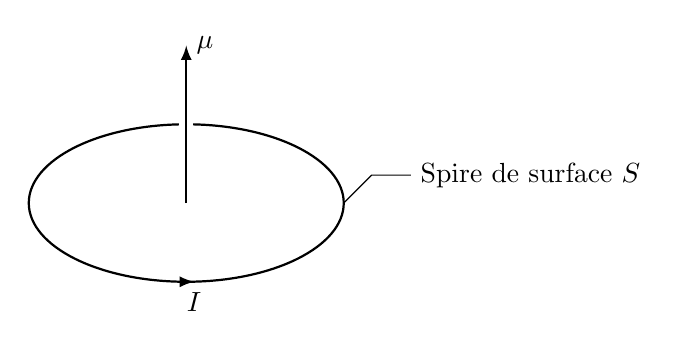
\begin{tikzpicture}
  %tikz  magnetisme
    \draw[thick] (0,0) ellipse[x radius=2cm,y radius=1cm];
    \draw[-latex, thick] (0, -1) -- ++(0.1,0) node[below] {$I$ };
    \draw[thick, -latex,preaction={draw, white, line width=5pt}] (0,0) -- ++(0,2) node[right]{$\vv{\mu}$ };
    \draw (2, 0) -- ++(45:0.5) -- ++(0.5, 0) node[right] {Spire de surface $S$ }; 
  \end{tikzpicture}
  \hspace{3em}
  \includegraphics[width=3cm]{images/regle_main_droite.pdf}

  \captionof{figure}{Moment magnétique associé à une spire et règle de la main droite pour déterminer son orientation.}
\end{center}
Par analogie, on associe également un moment magnétique à un aimant permanent. Pour les matériaux magnétiques, plutôt que de parler de moment magnétique, on donne plutôt leur aimantation $\vv{M} = \frac{\vv{\mu}}{V}$, où $\vv{\mu}$ est le moment magnétique et $V$ le volume du matériau, il s'agit du moment magnétique par unité de volume. L'aimantation des aimants permanents usuels (neodyme-fer-bore) est de l'ordre de \SI{1e6}{\ampere\per\meter}.
\end{document}
